% q0043.tex — Bubble Tea or Artisanal Coffee?
\question{
  id        = {0043},
  title     = {Bubble Tea or Artisanal Coffee?},
  source    = {OBECON},
  year      = {2026},
  round     = {Seletiva IEO -- Phase C},
  language  = {English},
  topic     = {Macro},
  subtopic  = {CPI / Index Numbers / Substitution Bias},
  type      = {objective},
  statement = {%
    Obeconomia debates CPI measurement methods. Method~L uses a fixed 2000
    basket (Laspeyres index); Method~P updates the basket annually (Paasche
    index). Between 2000 and 2025, bubble tea prices fell 30\% and artisanal
    coffee prices rose 40\%; all other prices remained unchanged.

    \begin{center}
      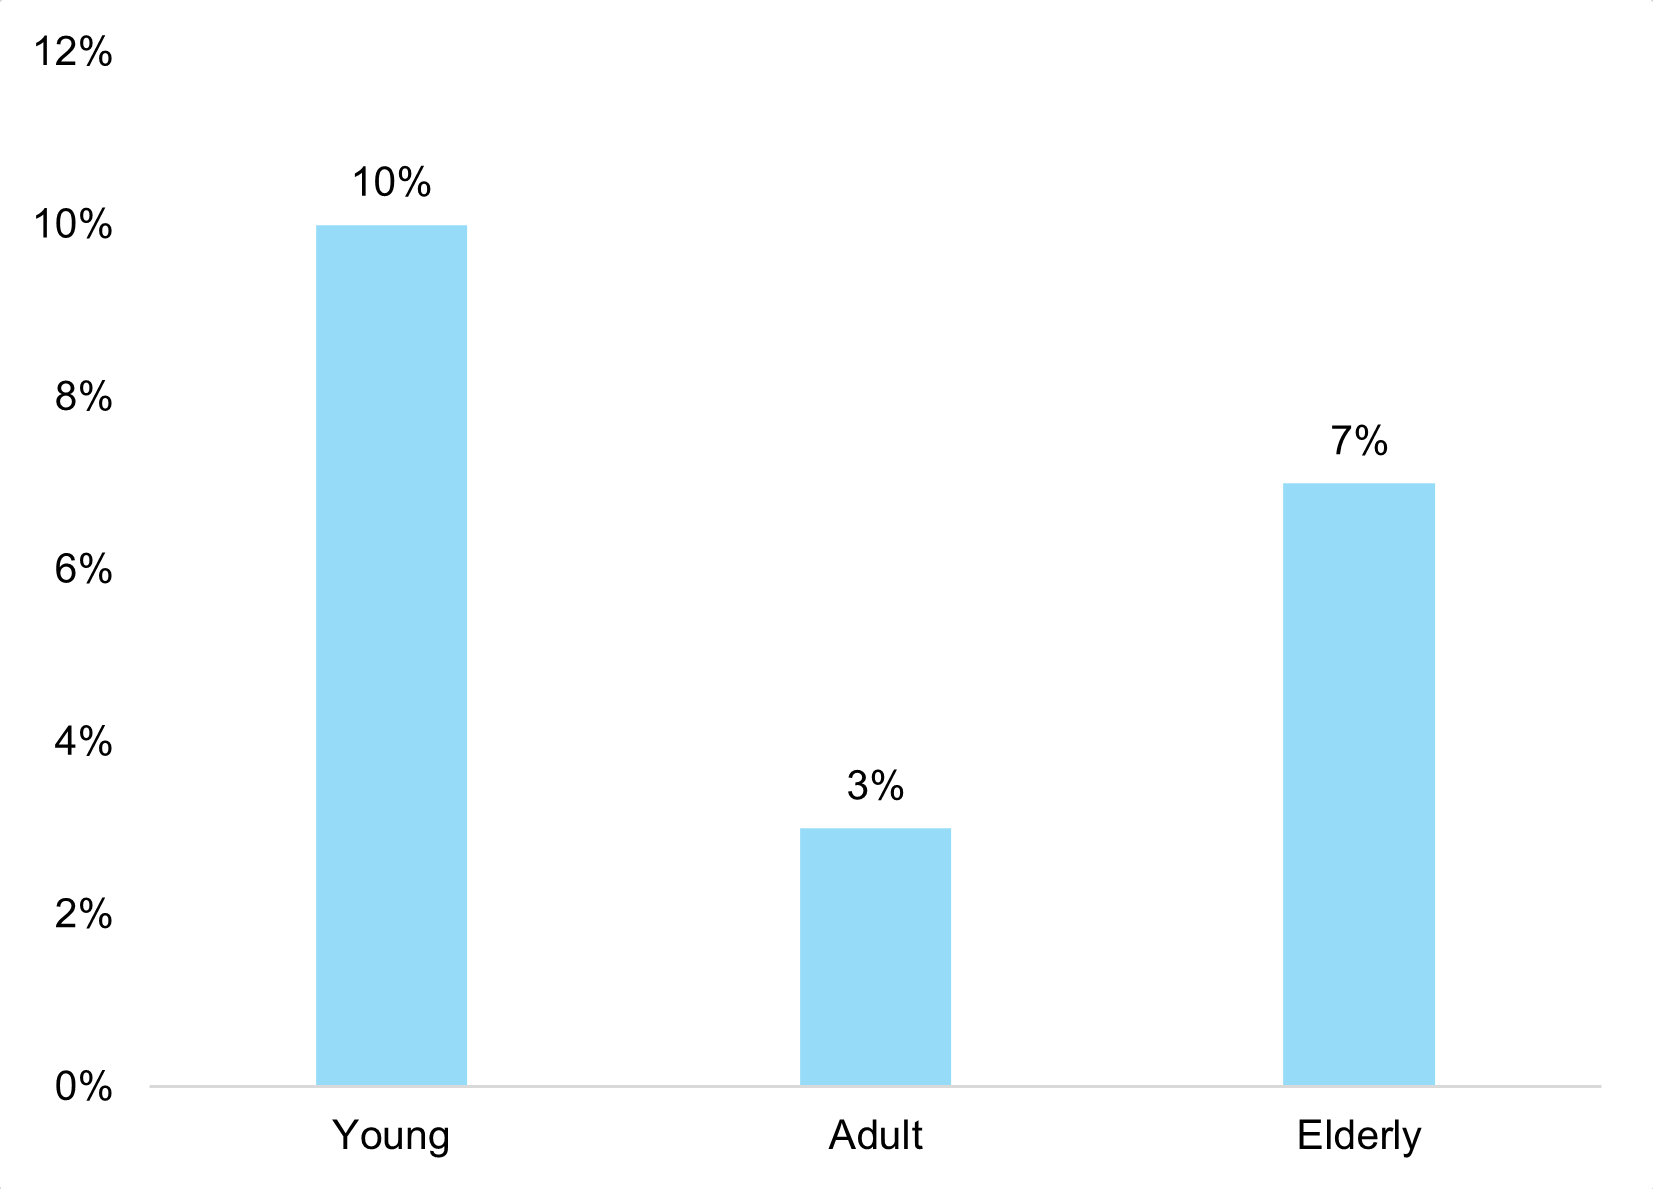
\includegraphics[width=0.75\textwidth]{../images/q0043_fig1.png}
    \end{center}

    Which comparison between the two indices is correct?
  },
  choices   = {%
    \item Both methods show identical inflation.
    \item The L-Index shows higher inflation than the P-Index due to
          substitution bias.
    \item The P-Index shows higher inflation than the L-Index due to
          substitution bias.
    \item The L-Index shows lower inflation than the P-Index because it uses
          outdated weights.
  },
  answer    = {B},
  solution  = {%
    The Laspeyres index overweights goods that have become relatively more
    expensive (artisanal coffee), while rational consumers substitute toward
    cheaper alternatives (bubble tea). This substitution bias causes
    $L \geq P$ mathematically. The fixed-basket L-Index therefore overstates
    inflation compared to the annually-updated P-Index. (B) is correct.
  },
}
